\documentclass[12pt, titlepage]{article}

\usepackage{fullpage}
\usepackage[round]{natbib}
\usepackage{multirow}
\usepackage{booktabs}
\usepackage{tabularx}
\usepackage{graphicx}
\usepackage{float}
\usepackage{hyperref}
\usepackage[shortlabels]{enumitem}
\usepackage{amsmath, mathtools}
\usepackage{amsfonts}
\usepackage{amssymb}
\usepackage{colortbl}
\usepackage{xr}
\usepackage{longtable}
\usepackage{xfrac}
\usepackage{siunitx}
\usepackage{caption}
\usepackage{pdflscape}
\usepackage{afterpage}
\usepackage{titlesec}
\usepackage{array}
%\usepackage{showframe}
\hypersetup{
    colorlinks,
    citecolor=blue,
    filecolor=black,
    linkcolor=red,
    urlcolor=blue
}
\usepackage{graphicx}
\graphicspath{ {./images/} }
\usepackage{caption}
\usepackage{enumitem}
\input{../Comments}
%% Common Parts

\newcommand{\progname}{Chess Connect} % PUT YOUR PROGRAM NAME HERE
\newcommand{\authname}{Team \#4,
\\ Alexander Van Kralingen
\\ Arshdeep Aujla
\\ Jonathan Cels
\\ Joshua Chapman
\\ Rupinder Nagra} % AUTHOR NAMES without MacIDs 

\usepackage{hyperref}
    \hypersetup{colorlinks=true, linkcolor=blue, citecolor=blue, filecolor=blue,
                urlcolor=blue, unicode=false}
    \urlstyle{same}

\newcommand{\projectoverview}{

The Chess Connect project allows two users to play a game of chess on a physical board with the information being transmitted to an online web application over Bluetooth.
Currently, there is no way for players to seamlessly switch between playing on a physical board and playing online, but Chess Connect intends to change this by creating a central platform that will provide flexibility and remove barriers for new players looking to learn the game.

}

\begin{document}

\title{System Verification and Validation Report for \progname{}} 
\author{\authname}
\date{\today}
	
\maketitle

\pagenumbering{roman}

\section{Revision History}

\begin{tabularx}{\textwidth}{p{3cm}p{2cm}X}
\toprule {\bf Date} & {\bf Version} & {\bf Notes}\\
\midrule
2023-03-04 & Arshdeep Aujla & Added Template for Nonfunctional Requirements\\
2023-03-05 & Arshdeep Aujla & Added Table for functional requirements, traceability matrix\\
2023-03-07 & Jonathan Cels & Added functional requirement test reports\\
\bottomrule
\end{tabularx}

~\newpage

\section{Symbols, Abbreviations and Acronyms}

\renewcommand{\arraystretch}{1.2}
\begin{tabular}{l l} 
  \toprule		
  \textbf{symbol} & \textbf{description}\\
  \midrule 
  T & Test\\
  \bottomrule
\end{tabular}\\

Refer to SRS Section 1 for an extensive list of used symbols, abbreviations, and acronyms.

\newpage

\tableofcontents

\listoftables %if appropriate

\listoffigures %if appropriate

\newpage

\pagenumbering{arabic}

This document ...

\section{Functional Requirements Evaluation}
Refer to the VnV Plan for descriptions of the tests derived to evaluate the functional requirements.
\subsection{Game Active State}

\begin{table}[H]
    \centering
        \setlength{\leftmargini}{0.4cm}
        \begin{tabular}{| >{\centering\arraybackslash}m{1cm} | 
            >{\centering\arraybackslash}m{2.5cm} | 
            >{\centering\arraybackslash}m{4cm} | 
            >{\centering\arraybackslash}m{3cm} |
            >{\centering\arraybackslash}m{3cm} |
            >{\centering\arraybackslash}m{1.5cm} |}
        \hline
        \rowcolor[gray]{0.9}
        Test & Input & Expected & Actual & Notes & Result\\
        \hline
        GA-1 & Draw/resign button pressed while game active. & System variable `gameInProgress' set to false. &  System variable configured correctly. &  & Pass \\
        \hline
        GA-2 & Start game button pressed while game active. & System variable `gameInProgress' remains true. &  System variable configured correctly. &  & Pass \\
        \hline
        GA-3 & User mode button pressed while game active. & System variable `currMode' changed to represent the selected user mode. &  User mode unchanged. & Design changed, user mode not switchable while a game is active. & Rework \\
        \hline
        GA-4 & Start game button pressed while game inactive. & System variable `gameInProgress' set to true, `currFEN' variable is set to the starting FEN. &  System variables configured correctly. &  & Pass \\
        \hline
        GA-5 & Move made that results in stalemate or checkmate according to the rules of chess while game inactive. & System variable `gameInProgress' set to false. &  System variable configured correctly. &  & Pass \\ 
        \hline
        \end{tabular}
    \caption{Active State Functional Requirements Results}
\end{table}

\subsection{Game Inactive State}

\begin{table}[H]
    \centering
        \setlength{\leftmargini}{0.4cm}
        \begin{tabular}{| >{\centering\arraybackslash}m{1cm} | 
            >{\centering\arraybackslash}m{2.5cm} | 
            >{\centering\arraybackslash}m{4cm} | 
            >{\centering\arraybackslash}m{3cm} |
            >{\centering\arraybackslash}m{3cm} |
            >{\centering\arraybackslash}m{1.5cm} |}
        \hline
        \rowcolor[gray]{0.9}
        Test & Input & Expected & Actual & Notes & Result\\
        \hline
        GI-1 & Start game button pressed while game inactive. & System variable `gameInProgress' set to true. & System variable configured correctly. &  & Pass \\
        \hline
        GI-2 & User mode button pressed while game inactive. & User mode unchanged. & System variable configured correctly. & Design changed, user mode is now switchable (only) while a game is inactive. & Rework \\
        \hline
        GI-3 & Draw/resign button pressed while game inactive. & System variable `gameInProgress' remains false. & System variable configured correctly. &  & Pass \\
        \hline
        GI-4 & Piece moved while game inactive. & System variable `currFEN' is unchanged. & System variable configured correctly. &  & Pass \\
        \hline
        GI-5 & Draw/resign button pressed, or move made that results in stalemate or checkmate according to the rules of chess while game active. & Game termination and winner are displayed on LCD screen. & Display updates correctly. &  & Pass \\
        \hline
        \end{tabular}
    \caption{Inactive State Functional Requirements Results}
\end{table}

\subsection{Normal Mode}

\begin{table}[H]
    \centering
        \setlength{\leftmargini}{0.4cm}
        \begin{tabular}{| >{\centering\arraybackslash}m{1cm} | 
            >{\centering\arraybackslash}m{2.5cm} | 
            >{\centering\arraybackslash}m{4cm} | 
            >{\centering\arraybackslash}m{3cm} |
            >{\centering\arraybackslash}m{3cm} |
            >{\centering\arraybackslash}m{1.5cm} |}
        \hline
        \rowcolor[gray]{0.9}
        Test & Input & Expected & Actual & Notes & Result\\
        \hline
        NB-1 & Piece moved while in normal mode. & Game state is updated to reflect piece movement. & Game state updated correctly. &  & Pass \\
        \hline
        NB-2 & Resign button pressed while in normal mode. & System variable `gameInProgress' set to false. & System variable configured correctly. &  & Pass \\
        \hline
        NB-3 & Draw button pressed while in normal mode. & System variable `gameInProgress' set to false. & System variable configured correctly. &  & Pass \\
        \hline
        ND-1 & Game state updated while in normal mode. & Updated game state is transmitted to the web application via Bluetooth. & Game state transmitted correctly. &  & Pass \\
        \hline
        NA-1 & Web application receives updated game state while in normal mode. & Update to game state is reflected on web application display. & Display updates correctly. &  & Pass \\
        \hline
        NA-2 & Game termination occurs while in normal mode. & Game termination and winner are displayed on web application display. & Display updates correctly. &  & Pass \\
        \hline
        \end{tabular}
    \caption{Normal Mode Functional Requirements Results}
\end{table}

\pagebreak
\subsection{Engine Mode}
    \begin{longtable}{| >{\centering\arraybackslash}m{1cm} | 
        >{\centering\arraybackslash}m{2.5cm} | 
        >{\centering\arraybackslash}m{4cm} | 
        >{\centering\arraybackslash}m{3cm} |
        >{\centering\arraybackslash}m{3cm} |
        >{\centering\arraybackslash}m{1.5cm} |}
    \hline
    \rowcolor[gray]{0.9}
    Test & Input & Expected & Actual & Notes & Result\\
    \hline
    EB-1 & Piece moved while in engine mode. & Game state is updated to reflect piece movement. & Game state updated correctly. &  & Pass \\
    \hline
    EB-2 & Resign button pressed while in engine mode. & System variable `gameInProgress' set to false. & System variable configured correctly. &  & Pass \\
    \hline
    EB-3 & Draw button pressed while in engine mode. & System variable `gameInProgress' set to false. & System variable configured correctly. &  & Pass \\
    \hline
    EB-4 & Engine moves transmitted from the web application to microcontroller. & Engine moves are displayed on the LCD screen. & Display updated correctly. &  & Pass \\
    \hline
    ED-1 & Game state updated while in engine mode. & Updated game state is transmitted to the web application via Bluetooth. & Game state transmitted correctly. &  & Pass \\
    \hline
    ED-2 & Engine moves are calculated by the web application. & Calculated engine moves are transmitted from the web application to the microcontroller via Bluetooth & Moves transmitted correctly. & Only one engine move currently calculated, more planned in future revisions. & Partial Pass \\
    \hline
    \pagebreak 
    \hline
    \rowcolor[gray]{0.9}
    Test & Input & Expected & Actual & Notes & Result\\
    \hline
    EA-1 & Web application receives updated game state while in engine mode. & Update to game state is reflected on web application display. & Display updates correctly. &  & Pass \\
    \hline
    EA-2 & Engine moves are calculated by the web application. & Calculated engine moves are displayed on web application display. & Engine moves are not displayed. & Not implemented, planned in future revisions. & TBD \\
    \hline
    EA-3 & Game termination occurs while in engine mode. & Game termination and winner are displayed on web application display. & Display updates correctly. &  & Pass \\
    \hline
    \caption{Engine Mode Functional Requirements Results}\\
\end{longtable}

\pagebreak

\subsection{Beginner Mode}
    \begin{longtable}{| >{\centering\arraybackslash}m{1cm} | 
        >{\centering\arraybackslash}m{2.5cm} | 
        >{\centering\arraybackslash}m{4cm} | 
        >{\centering\arraybackslash}m{3cm} |
        >{\centering\arraybackslash}m{3cm} |
        >{\centering\arraybackslash}m{1.5cm} |}
    \hline
    \rowcolor[gray]{0.9}
    Test & Input & Expected & Actual & Notes & Result\\
    \hline
    BB-1 & Piece moved while in beginner mode. & Game state is updated to reflect piece movement. & Game state updated correctly. &  & Pass \\
    \hline
    BB-2 & Piece picked up and held while in beginner mode. & LEDs on board indicate legal moves. & Correct LEDs light up. &  & Pass \\
    \hline
    BB-3 & Piece moved such that an illegal move is made while in beginner mode. & LEDs on board indicate illegal move. & Correct LEDs light up. & Not implemented, planned in future revisions. & TBD \\
    \hline
    BB-4 & Resign button is pressed while in beginner mode. & System variable `gameInProgress' set to false. & System variable configured correctly. &  & Pass \\
    \hline
    BB-5 & Draw button is pressed while in beginner mode. & System variable `gameInProgress' set to false. & System variable configured correctly. &  & Pass \\
    \hline
    BD-1 & Game state is updated while in beginner mode. & Updated game state is transmitted to the web application via Bluetooth. & Game state transmitted correctly. &  & Pass \\
    \hline
    \pagebreak 
    \hline
    \rowcolor[gray]{0.9}
    Test & Input & Expected & Actual & Notes & Result\\
    \hline
    BA-1 & User selcetions chess instructions in web application. & Web application displays detailed rules for how to play chess. & N/A & Not implemented, planned in future revisions. & TBD \\
    \hline
    BA-2 & Web application receives updated game state while in beginner mode. & Update to game state is reflected on web application display. & Display updates correctly. &  & Pass \\
    \hline
    \caption{Beginner Mode Functional Requirements Results}\\
\end{longtable}
    
\pagebreak

\section{Nonfunctional Requirements Evaluation}

Many of the nonfunctional requirements outlined in the VnV plan are left for revision 1, as much of the external testing relies on the product being more completed and accessible to a wider audience.
Some external user testing was done, specifically for NFT-4 and NFT-5, and is detailed in the Performance section.

\subsection{Look and Feel}

Look and feel testing will be performed for revision 1, as though it is functional, this part of the product is not ready for external user testing.
		
\subsection{Usability and Humanity}

Usability testing will be performed for revision 1, as though it is functional, this part of the product is not ready for external user testing.

\subsection{Performance}

\begin{table}[H]
    \centering
        \setlength{\leftmargini}{0.4cm}
        \begin{tabular}{| >{\centering\arraybackslash}m{2cm} | 
            >{\centering\arraybackslash}m{2.5cm} | 
            >{\centering\arraybackslash}m{3cm} | 
            >{\centering\arraybackslash}m{2cm} |
            >{\centering\arraybackslash}m{4cm} |
            >{\centering\arraybackslash}m{1.5cm} |}
        \hline
        \rowcolor[gray]{0.9}
        Test & Input & Expected & Actual & Notes & Result\\
        \hline
        NFT-4 & Experiment performed as detailed below. & Average LED response time over all trials is less than 0.5 seconds. & Average response time was 0.488 seconds. & This value is close to the 0.5 second limit, and may be subject to human error. Further testing will be done with more trials for revision 1 to ensure this requirement is met. & Pass \\
        \hline
        NFT-5 & Experiment performed as detailed below. & Maximum single response time of any trial is less than 1 second. & Maximum response time was 0.72 seconds. &  & Pass \\
        \hline
        NFT-6 & N/A & N/A & N/A & Not tested, as the system is currently subject to a 2-second delay before refreshing. Will be tested for revision 1. & TBD \\
        \hline
        NFT-7 & N/A & N/A & N/A & Not tested, as the system is currently subject to a 2-second delay before refreshing. Will be tested for revision 1. & TBD \\
        \hline
        \end{tabular}
    \caption{Performance Non-Functional Requirements Results}
\end{table}

\newpage
The following table holds data for NFT-4 and NFT-5. Three external users, all familiar with the rules of chess, were each asked to perform the following experiment in beginner mode 5 times:
\medskip
\\
Pick up an arbitrary piece and suspend it in the air. Wait until the board visually indicates the possible moves for the suspended piece. The time between the user picking up 
the piece and the board's LED indicators turning on was measured and recorded.

\begin{table}[H]
    \centering
    \setlength{\leftmargini}{0.4cm}
    \begin{tabular}{| >{\centering\arraybackslash}m{4cm} | 
        >{\centering\arraybackslash}m{3cm} |
        >{\centering\arraybackslash}m{3cm} | 
        >{\centering\arraybackslash}m{3cm} |}
    \hline
    \rowcolor[gray]{0.9}
    & User 1 & User 2 & User 3 \\
    \hline
    Trial 1 & 0.49s & 0.48s & 0.36s \\
    \hline
    Trial 2 & 0.65s & 0.69s & 0.27s \\
    \hline
    Trial 3 & 0.53s & 0.33s & 0.52s \\
    \hline
    Trial 4 & 0.72s & 0.34s & 0.49s \\
    \hline
    Trial 5 & 0.42s & 0.51s & 0.52s \\
    \hline
    Total Average & \multicolumn{3}{c|}{\textbf{0.488s}}\\
    \hline
    \end{tabular}
\caption{Experimental Results of Performance Testing}
\end{table}

The following scatter plot shows the experimental results visually. The average, shown in green, falls just below the 
required 0.5 second threshold, and all points are well below the maximum acceptable response time of 1 second.

\begin{figure}[H]
    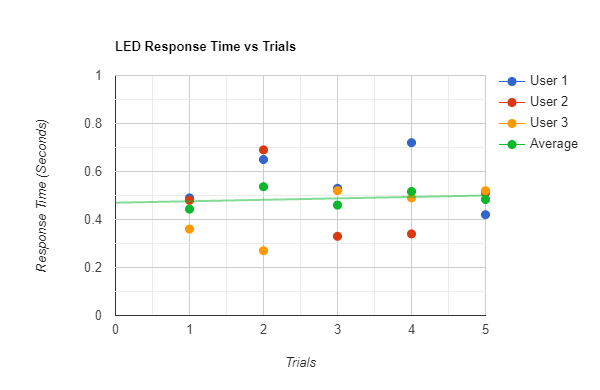
\includegraphics[scale=0.93]{performanceScatterPlot}
    \caption{Experimental Results of Performance Testing}
\end{figure}

\newpage
\subsection{Health and Safety}

\begin{table}[H]
\centering
    \setlength{\leftmargini}{0.4cm}
    \begin{tabular}{| >{\centering\arraybackslash}m{1cm} | 
        >{\centering\arraybackslash}m{4cm} | 
        >{\centering\arraybackslash}m{3cm} | 
        >{\centering\arraybackslash}m{3cm} |
        >{\centering\arraybackslash}m{2.5cm} |
        >{\centering\arraybackslash}m{1.5cm} |}
    \hline
    \rowcolor[gray]{0.9}
    Test & Input & Expected & Actual & Notes & Result\\
    \hline
    NFT-8 & 10 sample wires were chosen while the product was running. Their current and voltage were measured, and power was calculated using those measurements. & All power measurements below safe limits. & All power measurements below safe limits. & Measurements far below any safety thresholds. & Pass \\
    \hline
    \end{tabular}
\caption{Health and Safety Non-Functional Requirements Results}
\end{table}

The following table holds data for NFT-8. 

\begin{table}[H]
    \centering
    \setlength{\leftmargini}{0.4cm}
    \begin{tabular}{| >{\centering\arraybackslash}m{1cm} | 
        >{\centering\arraybackslash}m{3cm} |
        >{\centering\arraybackslash}m{1.5cm} | 
        >{\centering\arraybackslash}m{2cm} |
        >{\centering\arraybackslash}m{2cm} |
        >{\centering\arraybackslash}m{2.5cm} |
        >{\centering\arraybackslash}m{2.5cm} |}
    \hline
    \rowcolor[gray]{0.9}
    Wire \# & Wire Description & Gauge & Current (Amps) & Voltage (Volts) & Calculated Power (Watts) & Maximum power (Watts) \\
    \hline
    1 & Hall sensor 1 with black piece & 20 & 0.04 & 1.6 & 0.064 & 7.5 \\
    \hline
    2 & Hall sensor 32 with no piece & 20 & 0.03 & 1 & 0.03 & 7.5 \\
    \hline
    3 & Hall sensor 64 with white piece & 20 & 0.02 & 0.6 & 0.012 & 7.5 \\
    \hline
    4 & Arduino power line & 10 & 0.5 & 5 & 2.5 & 75 \\
    \hline
    5 & ADC 1 & 20 & 0.01 & 5 & 0.05 & 7.5 \\
    \hline
    6 & ADC 4 & 20 & 0.02 & 5 & 0.1 & 7.5 \\
    \hline
    7 & ADC clock & 20 & 0.05 & 5 & 0.25 & 7.5 \\
    \hline
    8 & Wall power supply (L) & 8 & 0.75 & 110 & 47.631 & 120 \\
    \hline
    9 & Wall power supply (G) & 8 & 0.01 & 0 & 0 & 120 \\
    \hline
    10 & Bluetooth RX & 20 & 0.02 & 5 & 0.1 & 7.5 \\
    \hline
    \end{tabular}
\caption{Experimental Results of Health and Safety Testing}
\end{table}

\subsection{Precision and Accuracy}

Precision and accuracy testing will be performed for revision 1, as though it is functional, this part of the product is not ready for external user testing.

\subsection{Capacity}

\begin{table}[H]
\centering
    \setlength{\leftmargini}{0.4cm}
    \begin{tabular}{| >{\centering\arraybackslash}m{1cm} | 
        >{\centering\arraybackslash}m{2.5cm} | 
        >{\centering\arraybackslash}m{4cm} | 
        >{\centering\arraybackslash}m{3cm} |
        >{\centering\arraybackslash}m{3cm} |
        >{\centering\arraybackslash}m{1.5cm} |}
    \hline
    \rowcolor[gray]{0.9}
    Test & Input & Expected & Actual & Notes & Result\\
    \hline
    NFT-10 & A relatively complex chess FEN position was transmitted via Bluetooth to the web application while in engine mode. & The measured memory usage of the web application is less than 1GB. & The maximum measured memory value was 1187.4 MB, as measured by Windows task manager. & Memory usage will increase in future revisions, as more engine moves will be calculated at a higher depth. & Pass \\
    \hline
    \end{tabular}
\caption{Capacity Non-Functional Requirements Results}
\end{table}

\subsection{Security}

\begin{table}[H]
\centering
    \setlength{\leftmargini}{0.4cm}
    \begin{tabular}{| >{\centering\arraybackslash}m{1cm} | 
        >{\centering\arraybackslash}m{2.5cm} | 
        >{\centering\arraybackslash}m{4cm} | 
        >{\centering\arraybackslash}m{3cm} |
        >{\centering\arraybackslash}m{3cm} |
        >{\centering\arraybackslash}m{1.5cm} |}
    \hline
    \rowcolor[gray]{0.9}
    Test & Input & Expected & Actual & Notes & Result\\
    \hline
    NFT-11 & Bluetooth connection to web application severed. & Web application alert that the connection has been lost. & N/A & Not implemented, planned in future revisions. & TBD \\
    \hline
    NFT-12 & Power connection to system is severed, and then restored after a short time frame. & The game state data is stored in local memory and is unchanged after power is restored. & Game state data is properly stored. &  & Pass \\
    \hline
    \end{tabular}
\caption{Security Non-Functional Requirements Results}
\end{table}

\section{Unit Testing}

\section{Changes Due to Testing}

\section{Automated Testing}
		
\section{Trace to Requirements}

\begin{longtable}{| p{.20\textwidth} | p{.80\textwidth} |}
  \hline
  Test & Requirement\\
  \hline
  GA-1 & GA1\\
  \hline
  GA-2 & GA2\\
  \hline
  GA-3 & GA3\\
  \hline
  GA-4 & GA6\\
  \hline
  GA-5 & GA7\\
  \hline
  GI-1 & GI1\\
  \hline
  GI-2 & GI2\\
  \hline
  GI-3 & GI3\\
  \hline
  GI-4 & GI4\\
  \hline
  GI-5 & GI5, GI6\\
  \hline
  NB-1 & NB1\\
  \hline
  NB-2 & NB2\\
  \hline
  NB-3 & NB3\\
  \hline
  ND-1 & ND1\\
  \hline
  NA-1 & NA1, NA2\\
  \hline
  NA-2 & NA3\\
  \hline
  EB-1 & EB1\\
  \hline
  EB-2 & EB2\\
  \hline
  EB-3 & EB3\\
  \hline
  EB-4 & EB4\\
  \hline
  ED-1 & ED1\\
  \hline
  ED-2 & ED2\\
  \hline
  EA-1 & EA1, EA2\\
  \hline
  EA-2 & EA3, EA4, EA5\\
  \hline
  EA-3 & EA6\\
  \hline
  BB-1 & BB1\\
  \hline
  BB-2 & BB2\\
  \hline
  BB-3 & BB3\\
  \hline
  BB-4 & BB4\\
  \hline
  BB-5 & BB5\\
  \hline
  BD-1 & BD1\\
  \hline
  BA-1 & BA1\\
  \hline
  BA-2 & BA2\\
  \hline
  NFT1 & LF3\\
  \hline
  NFT2 & UH5\\
  \hline
  NFT3 & UH6\\
  \hline
  NFT4 & PR1\\
  \hline
  NFT5 & PR2\\
  \hline
  NFT6 & PR3\\
  \hline
  NFT7 & PR4\\
  \hline
  NFT8 & PR6\\
  \hline
  NFT9 & PR7\\
  \hline
  NFT10 & PR10\\
  \hline
  NFT11 & SR4\\
  \hline
  NFT12 & SR3\\
  \hline
\caption{Requirements Traceability Matrix}
\end{longtable}
		
\section{Trace to Modules}		

\section{Code Coverage Metrics}

\appendix
\section{Reflection Appendix}


\bibliographystyle{plainnat}

\nocite{*}\bibliography{../../refs/References}

\end{document}